% Created 2020-06-01 Mon 17:58
% Intended LaTeX compiler: pdflatex
% Template: Diogo Ferrari
\documentclass[a4paper]{article}
% === Packages =================================
\usepackage{./sty/basic-article}
\usepackage{./sty/math-commands}
\usepackage{./sty/math-commands-thm}
% === Document =================================
\author{Diogo Ferrari\\
Department of Political Science\\
University of California, Riverside\\
}
\date{\today}
\title{Diagrams using tikz}
\hypersetup{
 pdfauthor={Diogo Ferrari\\
Department of Political Science\\
University of California, Riverside\\
},
 pdftitle={Diagrams using tikz},
 pdfkeywords={},
 pdfsubject={},
 pdfcreator={Emacs 26.3 (Org mode 9.0.9)}, 
 pdflang={English}}
\begin{document}

\maketitle
\tableofcontents

\pagebreak
\section{Instructions and Information}
\label{sec:orge628d2a}

To draw this diagrams, you need to use the following latex packages:
\begin{itemize}
\item \texttt{\textbackslash{}usepackage\{tikz\}}
\item \texttt{\textbackslash{}usetikzlibrary\{decorations.pathreplacing\}}
\item \texttt{\textbackslash{}usepackage\{forest\}}
\item \textbf{Note:} you may need additional packages. The file \texttt{./sty/basic-article.sty} contains all the packages you need and some extra ones.
\item You also need to create \texttt{./sty/}, save the file \texttt{math-commands.sty} on that folder, and include \texttt{\textbackslash{}usepackage\{./sty/math-commands\}} in your main file.
\end{itemize}

You can check the \texttt{.tex} file used to create this \texttt{.pdf} for details.

The diagrams created here uses the package \texttt{tikz}. See documentation \href{https://ctan.org/pkg/pgf?lang=en}{here}. It extends that package using commands whose deetails you can find \href{https://github.com/jluttine/tikz-bayesnet}{here}. The full code is in the appendix \ref{ap-settings} below, which is also in the file \texttt{math-commands.sty}.


\section{Nodes}
\label{sec:org0befa40}
\subsection{Basic shapes}
\label{sec:org32a261b}
Some predefined nodes on \texttt{basic-math-commands.sty}

\begin{figure}[ht]
\begin{tikzpicture}
  %% 
\node at (0, 5) [const  , label=right:const  (constant node)         ] (c) {\( c \)} ; %
\node at (5, 5) [caption,                                              ] (c-snippet) {(Snippet: dagnc)} ; %
%% 
\node at (0, 4) [latent, label=right:latent (latent node)           ] (z) {\( Z_i \)} ; %
\node at (5, 4) [caption,                                              ] () {(Snippet: dagnl)} ; %
%% 
\node at (0, 3) [obs   , label=right:obs    (observed node)         ] (x)  {\(X_i \)} ; %
\node at (5, 3) [caption,                                              ] () {(Snippet: dagno)} ; %
%% 
\node at (0, 2) [factor, label=right:factor (factor node)] (fa)  {$\beta$} ; %
\node at (5, 2) [caption,                                              ] () {(Snippet: dagnf)} ; %
%% 
\node at (0, 1) [factor, label=right:dist (distribution node)] (fa)  {$\beta$} ; %
\node at (5, 1) [caption,                                              ] () {(Snippet: dagndist)} ; %
%% 
\node at (0, 0) [det   , label=right:det    (deterministic node)    ] (det)  {$a$} ; %
\node at (5, 0) [caption,                                              ] () {(Snippet: dagnd)} ; %
%% 
\node at (0, -1) [operation   , label=right:operation    (operation node)    ] (det)  {\( \norm{\cdot}   \)} ; %
\node at (5, -1) [caption,                                              ] () {(Snippet: dagno)} ; %
\end{tikzpicture}
\end{figure}


\subsection{Template}
\label{sec:org83205e6}

\lstset{numbers=left,language=[LaTeX]TeX,label= ,caption= ,captionpos=b}
\begin{lstlisting}
\node at (<x>, <y>) [<properties>] (<node-id>) {<label>} ; %
\end{lstlisting}

\begin{description}
\item[{\color{red} <x> \color{black} and \color{red} <y> \color{black}}] position of the nodes
\item[{\color{red} <properties> \color{black}}] \begin{description}
\item[{circle, retangle, diamond}] shape (e.g., circle)
\item[{draw         }] color of the border (default draw=black)
\item[{minimum size }] minimum size of the node
\item[{inner sep    }] separation between label and node
\item[{font         }] font size
\item[{colorfont    }] font color (default=black)
\item[{fill         }] color to fill the node (default color=white)
\item[{node distance}] distange betweeen nodes
\item[{label=\{[<color>]<position>:\normalsize<text>\}        }] label next to node (e.g., label=right:"this node is about X"; <position> can be right, left, top, bottom, top right, etc.)
\end{description}
\item[{\color{red} <node-id> \color{black}}] label to identify the node
\item[{\color{red} <label> \color{black}}] text that appear inside the node
\end{description}

\subsection{Examples}
\label{sec:orgfea1b55}
\lstset{numbers=left,language=[LaTeX]TeX,label= ,caption= ,captionpos=b}
\begin{lstlisting}
\begin{figure}[ht]\centering
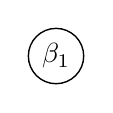
\begin{tikzpicture}
\node at (0, 0) [
  circle,                     % rectangle/diamond
  draw          = black,      % border
  line width    = .5pt,       % border width
  minimum size  = 20pt,       % minimum size of node
  inner sep     = 1pt,        % sep b/w border and inner text
  font          = \normalsize,%
  text          = black,      % inner label color
  fill          = white,
  node distance = 1pt,
  ]
  (beta1)
  {\( \beta_{1}  \)} ;
\end{tikzpicture}
\end{figure}
\end{lstlisting}

\begin{figure}[ht]\centering
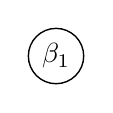
\begin{tikzpicture}
\node at (0, 0) [
  circle,                     % rectangle/diamond
  draw          = black,      % border
  line width    = .5pt,       % border width
  minimum size  = 20pt,       % minimum size of node
  inner sep     = 1pt,        % sep b/w border and inner text
  font          = \normalsize,%
  text          = black,      % inner label color
  fill          = white,
  node distance = 1pt,
  ]
  (beta1)
  {\( \beta_{1}  \)} ;
\end{tikzpicture}
\end{figure}


\lstset{numbers=left,language=[LaTeX]TeX,label= ,caption= ,captionpos=b}
\begin{lstlisting}
\begin{figure}[ht]\centering
\begin{tikzpicture}
\node at (0, 0) [
  circle,                     % rectangle/diamond
  draw          = black,      % border
  line width    = .5pt,       % border width
  minimum size  = 20pt,       % minimum size of node
  inner sep     = 1pt,        % sep b/w border and inner text
  font          = \normalsize,%
  text          = black,      % inner label color
  fill          = white,
  node distance = 1pt,
  ]
  (beta1)
  {\( \beta_{1}  \)} ; %
\node at (1, 0) [
  circle,                     % rectangle/diamond
  draw          = black,      % border
  ]
  ()
  {\( \Sigma  \)} ;
\node at (3, 0) [latent ] (id) {<label>} ; %
\node at (5, 0) [obs    ] (mu) {\( \mu  \)} ; %
\node at (7, 0) [const  ] (id-x) {X} ; %
\end{tikzpicture}
\end{figure}
\end{lstlisting}

\begin{figure}[ht]\centering
\begin{tikzpicture}
\node at (0, 0) [
  circle,                     % rectangle/diamond
  draw          = black,      % border
  line width    = .5pt,       % border width
  minimum size  = 20pt,       % minimum size of node
  inner sep     = 1pt,        % sep b/w border and inner text
  font          = \normalsize,%
  text          = black,      % inner label color
  fill          = white,
  node distance = 1pt,
  ]
  (beta1)
  {\( \beta_{1}  \)} ; %
\node at (1, 0) [
  circle,                     % rectangle/diamond
  draw          = black,      % border
  ]
  ()
  {\( \Sigma  \)} ;
\node at (3, 0) [latent ] (id) {<label>} ; %
\node at (5, 0) [obs    ] (mu) {\( \mu  \)} ; %
\node at (7, 0) [const  ] (id-x) {X} ; %
\end{tikzpicture}
\end{figure}


\section{Plate and Parametric Models}
\label{sec:org928d656}

\subsection{Basic shapes}
\label{sec:org26cf561}

\begin{figure}[ht]\centering
\begin{tikzpicture}
\node at (0, 0) [latent ] (a) {a} ; %
\node at (2, 0) [latent ] (b) {b} ; %
\node at (4, 1) [latent ] (c) {c} ; %
\node at (6, 1) [latent ] (d) {d} ; %
\node at (2,-1) [latent ] (e) {e} ; %
%% 
\plate [solid]   {plate1} {(e) (b)} {}; %
\plate [dashed]  {plate2} {(a) (c)} {\( i=1,..., n \)}; %
\plate [dotted]  {plate3} {(c) (d)} {N}; %
\end{tikzpicture}
\end{figure}


\subsection{Examples}
\label{sec:org7aa290e}

\lstset{numbers=left,language=[LaTeX]TeX,label= ,caption= ,captionpos=b}
\begin{lstlisting}
\begin{figure}[ht]\centering
\begin{tikzpicture}[thick,scale=1, every node/.style={transform shape}]
%% Nodes
\node at (2, 0) [obs        ] (yi)         {\( y_i \)} ; %
\node at (0, 0) [latent     ] (fi)         {\( f_i \)} ; %
\node at (-2, 0) [latent    ] (betai)      {\( \beta_ {i}  \)} ; %
\node at (-2, 2) [const     ] (Sigmabeta)  {\( \Sigma_{\beta }  \)} ; %
\node at (-4, 0) [const    ] (mubeta)     {\( \mu_   {\beta }  \)} ; %
\node at (0, 2) [latent     ] (theta)      {\( \theta  \)} ; %
\node at (-1, 4) [const     ] (mutheta)    {\( \mu_   {\theta } =0 \)} ; %
\node at ( 1, 4) [const     ] (Sigmatheta) {\( \Sigma_{\theta }=I   \)} ; %
\node at (-1, -2.5) [const  ] (l)          {\( l=1 \)} ; %
\node at ( 1, -2.5) [const  ] (sigmaf)     {\( \sigma_{f} =1 \)} ; %

%% plate
\plate {plate1} {(betai) (fi) (yi)} {\( i=1,...n \)}; 

%% arrows
\edge {fi} {yi}
\edge {betai} {fi}
\edge {mubeta} {betai}
\edge {l} {fi}
\edge {sigmaf} {fi}
\edge {Sigmabeta} {betai}
\edge {mutheta} {theta}
\edge {Sigmatheta} {theta}
\edge {theta} {fi}
\end{tikzpicture}
\end{figure}
\end{lstlisting}

\begin{figure}[ht]\centering
\begin{tikzpicture}[thick,scale=1, every node/.style={transform shape}]
%% Nodes
\node at (2, 0) [obs        ] (yi)         {\( y_i \)} ; %
\node at (0, 0) [latent     ] (fi)         {\( f_i \)} ; %
\node at (-2, 0) [latent    ] (betai)      {\( \beta_ {i}  \)} ; %
\node at (-2, 2) [const     ] (Sigmabeta)  {\( \Sigma_{\beta }  \)} ; %
\node at (-4, 0) [const    ] (mubeta)     {\( \mu_   {\beta }  \)} ; %
\node at (0, 2) [latent     ] (theta)      {\( \theta  \)} ; %
\node at (-1, 4) [const     ] (mutheta)    {\( \mu_   {\theta } =0 \)} ; %
\node at ( 1, 4) [const     ] (Sigmatheta) {\( \Sigma_{\theta }=I   \)} ; %
\node at (-1, -2.5) [const  ] (l)          {\( l=1 \)} ; %
\node at ( 1, -2.5) [const  ] (sigmaf)     {\( \sigma_{f} =1 \)} ; %

%% plate
\plate {plate1} {(betai) (fi) (yi)} {\( i=1,...n \)}; 

%% arrows
\edge {fi} {yi}
\edge {betai} {fi}
\edge {mubeta} {betai}
\edge {l} {fi}
\edge {sigmaf} {fi}
\edge {Sigmabeta} {betai}
\edge {mutheta} {theta}
\edge {Sigmatheta} {theta}
\edge {theta} {fi}
\end{tikzpicture}
\end{figure}


\lstset{numbers=left,language=[LaTeX]TeX,label= ,caption= ,captionpos=b}
\begin{lstlisting}
\begin{figure}[ht]\centering
\begin{tikzpicture}[thick,scale=1, every node/.style={transform shape}, on grid, auto]
%% Nodes
\node at (-6, 0) [const                ] (mubeta)      {\( \mu_   {\beta }  \)} ; %
\node at (-4, 2) [const                ] (Sigmabeta)  {\( \Sigma_{\beta }  \)} ; %
\node at (-4, 0) [dist, label={[red    ]below:\normalsize\( \No \)}  ] (normal)  {} ; %
\node at (2, 0) [obs                   ] (yi)         {\( y_i \)} ; %
\node at (0, 0) [latent                ] (fi)         {\( f_i \)} ; %
\node at (-2, 0) [latent               ] (betai)      {\( \beta_ {i}  \)} ; %
\node at (0, 2) [latent                ] (theta)      {\( \theta  \)} ; %
\node at (-1, 5) [const                ] (mutheta)    {\( \mu_   {\theta } =0 \)} ; %
\node at ( 1, 5) [const                ] (Sigmatheta) {\( \Sigma_{\theta }	=I   \)} ; %
\node at (-1, -4) [const             ] (l)          {\( l				=1 \)} ; %
\node at ( 1, -4) [const             ] (sigmaf)     {\( \sigma_{f}		=1 \)} ; %
\node at (0, -2.5) [dist, label={[black]right:\normalsize \( \G \)}  ] (g)  {} ; % 
\node at (2, 2) [operation             ] (dot) {\( \norm{.}   \)} ; %
\node at (4, 3) [latent                ] (x) {\( X \)} ; %
\node at (4, 1) [latent                ] (z) {\( Z \)} ; %
\node at (0, 3.5) [dist, label={[black]right:\normalsize\( \No \)}  ] (normaltheta)  {} ; % 
%% arrows
\edge [-] {mubeta} {normal}
\edge [-] {Sigmabeta} {normal}
\edge {normal} {betai} ;
\edge {fi} {yi}
\edge {betai} {fi}
\edge [-] {l} {g}
\edge [-] {sigmaf} {g}
\edge {g} {fi} ;
\edge [-] {mutheta} {normaltheta}
\edge [-] {Sigmatheta} {normaltheta}
\edge {normaltheta} {theta} ;
\edge {theta} {fi}
\edge [-] {x} {dot} ;
\edge [-] {z} {dot} ;
\edge {dot} {theta} ;

%% plate
\plate {plate1} {(betai) (fi) (yi)} {\( i=1,...n \)}; 
\end{tikzpicture}
\end{figure}
\end{lstlisting}

\begin{figure}[ht]\centering
\begin{tikzpicture}[thick,scale=1, every node/.style={transform shape}, on grid, auto]
%% Nodes
\node at (-6, 0) [const                ] (mubeta)      {\( \mu_   {\beta }  \)} ; %
\node at (-4, 2) [const                ] (Sigmabeta)  {\( \Sigma_{\beta }  \)} ; %
\node at (-4, 0) [dist, label={[red    ]below:\normalsize\( \No \)}  ] (normal)  {} ; %
\node at (2, 0) [obs                   ] (yi)         {\( y_i \)} ; %
\node at (0, 0) [latent                ] (fi)         {\( f_i \)} ; %
\node at (-2, 0) [latent               ] (betai)      {\( \beta_ {i}  \)} ; %
\node at (0, 2) [latent                ] (theta)      {\( \theta  \)} ; %
\node at (-1, 5) [const                ] (mutheta)    {\( \mu_   {\theta } =0 \)} ; %
\node at ( 1, 5) [const                ] (Sigmatheta) {\( \Sigma_{\theta }	=I   \)} ; %
\node at (-1, -4) [const             ] (l)          {\( l				=1 \)} ; %
\node at ( 1, -4) [const             ] (sigmaf)     {\( \sigma_{f}		=1 \)} ; %
\node at (0, -2.5) [dist, label={[black]right:\normalsize \( \G \)}  ] (g)  {} ; % 
\node at (2, 2) [operation             ] (dot) {\( \norm{.}   \)} ; %
\node at (4, 3) [latent                ] (x) {\( X \)} ; %
\node at (4, 1) [latent                ] (z) {\( Z \)} ; %
\node at (0, 3.5) [dist, label={[black]right:\normalsize\( \No \)}  ] (normaltheta)  {} ; % 
%% arrows
\edge [-] {mubeta} {normal}
\edge [-] {Sigmabeta} {normal}
\edge {normal} {betai} ;
\edge {fi} {yi}
\edge {betai} {fi}
\edge [-] {l} {g}
\edge [-] {sigmaf} {g}
\edge {g} {fi} ;
\edge [-] {mutheta} {normaltheta}
\edge [-] {Sigmatheta} {normaltheta}
\edge {normaltheta} {theta} ;
\edge {theta} {fi}
\edge [-] {x} {dot} ;
\edge [-] {z} {dot} ;
\edge {dot} {theta} ;

%% plate
\plate {plate1} {(betai) (fi) (yi)} {\( i=1,...n \)}; 
\end{tikzpicture}
\end{figure}

\section{DAG}
\label{sec:org70ab78b}
\subsection{Nodes as Text and box}
\label{sec:orga10a15b}
\lstset{numbers=left,language=[LaTeX]TeX,label= ,caption= ,captionpos=b}
\begin{lstlisting}
\begin{figure}[ht]\centering
\begin{tikzpicture}[thick,scale=1, every node/.style={transform shape}, on grid, auto]
\node at (0, 0)   [textnode, text width=2.5cm    ] (ind) {Socio-economic Positions} ; %
\node at (2.5, 2) [textnode, text width=1.8cm    ] (med) {Perceptions} ; %
\node at (5, 0)   [textnode, text width=2cm    ] (out) {Support for Populism} ; %

%% edges
\path[->] (ind)  edge node[el,left,rotate=0] {\( \lambda \quad \) }   (med);
\path[->] (med)  edge node[el,right,rotate=0] {\(\quad \beta  \)}   (out);
\path[->] (ind)  edge node[el,above,rotate=0] {\( \alpha  \)}   (out);
\end{tikzpicture}
\end{figure}
\end{lstlisting}

\begin{figure}[ht]\centering
\begin{tikzpicture}[thick,scale=1, every node/.style={transform shape}, on grid, auto]
\node at (0, 0)   [textnode, text width=2.5cm    ] (ind) {Socio-economic Positions} ; %
\node at (2.5, 2) [textnode, text width=1.8cm    ] (med) {Perceptions} ; %
\node at (5, 0)   [textnode, text width=2cm    ] (out) {Support for Populism} ; %

%% edges
\path[->] (ind)  edge node[el,left,rotate=0] {\( \lambda \quad \) }   (med);
\path[->] (med)  edge node[el,right,rotate=0] {\(\quad \beta  \)}   (out);
\path[->] (ind)  edge node[el,above,rotate=0] {\( \alpha  \)}   (out);
\end{tikzpicture}
\end{figure}

\subsection{Nodes as text}
\label{sec:org945abfa}

\lstset{numbers=left,language=[LaTeX]TeX,label= ,caption= ,captionpos=b}
\begin{lstlisting}
\begin{figure}[ht]\centering
\begin{tikzpicture}[thick,scale=1, every node/.style={transform shape}, on grid, auto]
\node at (0, 0)   [text width=2.5cm    ] (ind) {Socio-economic Positions} ; %
\node at (2.5, 2) [text width=1.8cm    ] (med) {Perceptions} ; %
\node at (5, 0)   [text width=2cm    ] (out) {Support for Populism} ; %

%% edges
\path[->] (ind)  edge node[el,left,rotate=0] {\( \lambda \quad \) }   (med);
\path[->] (med)  edge node[el,right,rotate=0] {\(\quad \beta  \)}   (out);
\path[->] (ind)  edge node[el,above,rotate=0] {\( \alpha  \)}   (out);
\end{tikzpicture}
\end{figure}
\end{lstlisting}

\begin{figure}[ht]\centering
\begin{tikzpicture}[thick,scale=1, every node/.style={transform shape}, on grid, auto]
\node at (0, 0)   [text width=2.5cm    ] (ind) {Socio-economic Positions} ; %
\node at (2.5, 2) [text width=1.8cm    ] (med) {Perceptions} ; %
\node at (5, 0)   [text width=2cm    ] (out) {Support for Populism} ; %

%% edges
\path[->] (ind)  edge node[el,left,rotate=0] {\( \lambda \quad \) }   (med);
\path[->] (med)  edge node[el,right,rotate=0] {\(\quad \beta  \)}   (out);
\path[->] (ind)  edge node[el,above,rotate=0] {\( \alpha  \)}   (out);
\end{tikzpicture}
\end{figure}

\subsection{Nodes as variables (relative position)}
\label{sec:org22dd295}

\lstset{numbers=left,language=[LaTeX]TeX,label= ,caption= ,captionpos=b}
\begin{lstlisting}
\begin{figure}[ht]\centering
\begin{tikzpicture}[thick,scale=1, every node/.style={transform shape}, on grid, auto]
\node at (0, 0)   [   ] (ind) {X} ; %
\node (med) [above right =  1.5cm and 1.5cm of ind] {Z};
\node (out) [right = 3cm and 3cm of ind] {Y} ; %

%% edges
\path[->] (ind)  edge node[el,left,rotate=0] {\( \lambda \quad \) }   (med);
\path[->] (med)  edge node[el,right,rotate=0] {\(\quad \beta  \)}   (out);
\path[->] (ind)  edge node[el,above,rotate=0] {\( \alpha  \)}   (out);
\end{tikzpicture}
\end{figure}
\end{lstlisting}

\begin{figure}[ht]\centering
\begin{tikzpicture}[thick,scale=1, every node/.style={transform shape}, on grid, auto]
\node at (0, 0)   [   ] (ind) {X} ; %
\node (med) [above right =  1.5cm and 1.5cm of ind] {Z};
\node (out) [right = 3cm and 3cm of ind] {Y} ; %

%% edges
\path[->] (ind)  edge node[el,left,rotate=0] {\( \lambda \quad \) }   (med);
\path[->] (med)  edge node[el,right,rotate=0] {\(\quad \beta  \)}   (out);
\path[->] (ind)  edge node[el,above,rotate=0] {\( \alpha  \)}   (out);
\end{tikzpicture}
\end{figure}

\subsection{Nodes as variables and circles}
\label{sec:org919748b}

\lstset{numbers=left,language=[LaTeX]TeX,label= ,caption= ,captionpos=b}
\begin{lstlisting}
\begin{figure}[ht]\centering
\begin{tikzpicture}[thick,scale=1, every node/.style={transform shape}, on grid, auto]
\node at (0, 0)   [latent     ] (ind) {X} ; %
\node at (2.5, 2) [latent,    ] (med) {Z} ; %
\node at (5, 0)   [latent,    ] (out) {Y} ; %

%% edges
\path[->] (ind)  edge node[el,left,rotate=0] {\( \lambda \quad \) }   (med);
\path[->] (med)  edge node[el,right,rotate=0] {\(\quad \beta  \)}   (out);
\path[->] (ind)  edge node[el,above,rotate=0] {\( \alpha  \)}   (out);
\end{tikzpicture}
\end{figure}
\end{lstlisting}

\begin{figure}[ht]\centering
\begin{tikzpicture}[thick,scale=1, every node/.style={transform shape}, on grid, auto]
\node at (0, 0)   [latent     ] (ind) {X} ; %
\node at (2.5, 2) [latent,    ] (med) {Z} ; %
\node at (5, 0)   [latent,    ] (out) {Y} ; %

%% edges
\path[->] (ind)  edge node[el,left,rotate=0] {\( \lambda \quad \) }   (med);
\path[->] (med)  edge node[el,right,rotate=0] {\(\quad \beta  \)}   (out);
\path[->] (ind)  edge node[el,above,rotate=0] {\( \alpha  \)}   (out);
\end{tikzpicture}
\end{figure}


\subsection{Nodes as variables and circles (closer)}
\label{sec:orgbed70c3}


\lstset{numbers=left,language=[LaTeX]TeX,label= ,caption= ,captionpos=b}
\begin{lstlisting}
\begin{figure}[ht]\centering
\begin{tikzpicture}[thick,scale=1, every node/.style={transform shape}, on grid, auto]
\node at (0, 0)   [latent     ] (ind) {X} ; %
\node at (2, 1.5) [latent,    ] (med) {Z} ; %
\node at (4, 0)   [latent,    ] (out) {Y} ; %

%% edges
\path[->] (ind)  edge node[el,left,rotate=0] {\( \lambda \quad \) }   (med);
\path[->] (med)  edge node[el,right,rotate=0] {\(\quad \beta  \)}   (out);
\path[->] (ind)  edge node[el,above,rotate=0] {\( \alpha  \)}   (out);
\end{tikzpicture}
\end{figure}
\end{lstlisting}

\begin{figure}[ht]\centering
\begin{tikzpicture}[thick,scale=1, every node/.style={transform shape}, on grid, auto]
\node at (0, 0)   [latent     ] (ind) {X} ; %
\node at (2, 1.5) [latent,    ] (med) {Z} ; %
\node at (4, 0)   [latent,    ] (out) {Y} ; %

%% edges
\path[->] (ind)  edge node[el,left,rotate=0] {\( \lambda \quad \) }   (med);
\path[->] (med)  edge node[el,right,rotate=0] {\(\quad \beta  \)}   (out);
\path[->] (ind)  edge node[el,above,rotate=0] {\( \alpha  \)}   (out);
\end{tikzpicture}
\end{figure}


\subsection{Nodes as variables and circles (closer, no edge labels)}
\label{sec:org7341cf9}


\lstset{numbers=left,language=[LaTeX]TeX,label= ,caption= ,captionpos=b}
\begin{lstlisting}
\begin{figure}[ht]\centering
\begin{tikzpicture}[thick,scale=1, every node/.style={transform shape}, on grid, auto]
\node at (0, 0)   [latent     ] (ind) {X} ; %
\node at (2, 1.5) [latent,    ] (med) {Z} ; %
\node at (4, 0)   [latent,    ] (out) {Y} ; %

%% edges
\path[->] (ind)  edge node[el,left,rotate=0]  {}   (med);
\path[->] (med)  edge node[el,right,rotate=0] {}   (out);
\path[->] (ind)  edge node[el,above,rotate=0] {}   (out);
\end{tikzpicture}
\end{figure}
\end{lstlisting}

\begin{figure}[ht]\centering
\begin{tikzpicture}[thick,scale=1, every node/.style={transform shape}, on grid, auto]
\node at (0, 0)   [latent     ] (ind) {X} ; %
\node at (2, 1.5) [latent,    ] (med) {Z} ; %
\node at (4, 0)   [latent,    ] (out) {Y} ; %

%% edges
\path[->] (ind)  edge node[el,left,rotate=0]  {}   (med);
\path[->] (med)  edge node[el,right,rotate=0] {}   (out);
\path[->] (ind)  edge node[el,above,rotate=0] {}   (out);
\end{tikzpicture}
\end{figure}

\subsection{Nodes as variables and circles (closer, no edge labels, and subfigures)}
\label{sec:org27abfba}

\lstset{numbers=left,language=[LaTeX]TeX,label= ,caption= ,captionpos=b}
\begin{lstlisting}
\begin{figure}[ht]
\begin{subfigure}{.5\textwidth}
  % ------------------------------
  \centering
  \begin{tikzpicture}[thick,scale=1, every node/.style={transform shape}, on grid, auto]
  \node at (0, 0)   [latent     ] (ind) {X} ; %
  \node at (2, 1.5) [latent,    ] (med) {Z} ; %
  \node at (4, 0)   [latent,    ] (out) {Y} ; %
  
  %% edges
  \path[->] (ind)  edge node[el,left,rotate=0]  {}   (med);
  \path[->] (med)  edge node[el,right,rotate=0] {}   (out);
  \path[->] (ind)  edge node[el,above,rotate=0] {}   (out);
  \end{tikzpicture}
  \caption{Put your sub-caption here}
  \label{fig:sub-first}
  % ------------------------------
\end{subfigure}
\begin{subfigure}{.5\textwidth}
  % ------------------------------
  \centering
  \begin{tikzpicture}[thick,scale=.7, every node/.style={transform shape}, on grid, auto]
  \node at (0, 0)   [latent     ] (ind) {X} ; %
  \node at (2, 1.5) [latent,    ] (med) {Z} ; %
  \node at (4, 0)   [latent,    ] (out) {Y} ; %
  
  %% edges
  \path[->] (ind)  edge node[el,left,rotate=0]  {}   (med);
  \path[<-] (med)  edge node[el,right,rotate=0] {}   (out);
  \path[->] (ind)  edge node[el,above,rotate=0] {}   (out);
  \end{tikzpicture}
  \caption{Put your sub-caption here}
  \label{fig:sub-second}
  % ------------------------------
\end{subfigure}
\caption{Put your caption here}
\label{fig:fig}
\end{figure}
\end{lstlisting}

\begin{figure}[ht]
\begin{subfigure}{.5\textwidth}
  % ------------------------------
  \centering
  \begin{tikzpicture}[thick,scale=1, every node/.style={transform shape}, on grid, auto]
  \node at (0, 0)   [latent     ] (ind) {X} ; %
  \node at (2, 1.5) [latent,    ] (med) {Z} ; %
  \node at (4, 0)   [latent,    ] (out) {Y} ; %
  
  %% edges
  \path[->] (ind)  edge node[el,left,rotate=0]  {}   (med);
  \path[->] (med)  edge node[el,right,rotate=0] {}   (out);
  \path[->] (ind)  edge node[el,above,rotate=0] {}   (out);
  \end{tikzpicture}
  \caption{Put your sub-caption here}
  \label{fig:sub-first}
  % ------------------------------
\end{subfigure}
\begin{subfigure}{.5\textwidth}
  % ------------------------------
  \centering
  \begin{tikzpicture}[thick,scale=.7, every node/.style={transform shape}, on grid, auto]
  \node at (0, 0)   [latent     ] (ind) {X} ; %
  \node at (2, 1.5) [latent,    ] (med) {Z} ; %
  \node at (4, 0)   [latent,    ] (out) {Y} ; %
  
  %% edges
  \path[->] (ind)  edge node[el,left,rotate=0]  {}   (med);
  \path[<-] (med)  edge node[el,right,rotate=0] {}   (out);
  \path[->] (ind)  edge node[el,above,rotate=0] {}   (out);
  \end{tikzpicture}
  \caption{Put your sub-caption here}
  \label{fig:sub-second}
  % ------------------------------
\end{subfigure}
\caption{Put your caption here}
\label{fig:fig}
\end{figure}

\subsection{Large DAG}
\label{sec:org3b5cc4d}

\begin{figure}[ht]\centering
\begin{tikzpicture}[thick,scale=1, every node/.style={transform shape}, on grid, auto]
\node at (0, 0) [] (x) {X} ;
\node[above right = 1.5cm and 1.5cm of x] (z) {Z};
\node[right = 3cm and 3cm of x] (y) {Y};
\node[above left = 1.5cm and 1.5cm of x] (u1) {\( U_1 \)};
\node[above right = 1.5cm and 1.5cm of u1] (u2) {\( U_2 \)};
%% edges
\edge {x} {y} ;
\edge {x} {z} ;
\edge {z} {y} ;
\edge {u1} {z} ;
\edge {u2} {z} ;
\edge {u2} {u1} ;
\edge {u1} {x} ;
\end{tikzpicture}
\end{figure}


\subsection{Large DAG (using latent var notation)}
\label{sec:org02b85a7}

\begin{figure}[ht]\centering
\begin{tikzpicture}[thick,scale=1, every node/.style={transform shape}, on grid, auto]
\node at (0, 0) [obs] (x) {X} ;
\node[obs, above right = 1.5cm and 1.5cm of x] (z) {Z};
\node[obs, right = 3cm and 3cm of x] (y) {Y};
\node[latent, above left = 1.5cm and 1.5cm of x] (u1) {\( U_1 \)};
\node[latent, above right = 1.5cm and 1.5cm of u1] (u2) {\( U_2 \)};
%% edges
\edge {x} {y} ;
\edge {x} {z} ;
\edge {z} {y} ;
\edge {u1} {z} ;
\edge {u2} {z} ;
\edge {u2} {u1} ;
\edge {u1} {x} ;
\end{tikzpicture}
\end{figure}


\subsection{Large DAG (using latent var notation alternative)}
\label{sec:org4691977}


\begin{figure}[ht]\centering
\begin{tikzpicture}[thick,scale=1, every node/.style={transform shape}, on grid, auto]
\node at (0, 0) [latent] (x) {X} ;
\node[latent, above right = 1.5cm and 1.5cm of x] (z) {Z};
\node[latent, right = 3cm and 3cm of x] (y) {Y};
\node[latent, dashed, above left = 1.5cm and 1.5cm of x] (u1) {\( U_1 \)};
\node[latent, dashed, above right = 1.5cm and 1.5cm of u1] (u2) {\( U_2 \)};
%% edges
\edge {x} {y} ;
\edge {x} {z} ;
\edge {z} {y} ;
\edge {u1} {z} ;
\edge {u2} {z} ;
\edge {u2} {u1} ;
\edge {u1} {x} ;
\end{tikzpicture}
\end{figure}

\section{Undirected Graphs}
\label{sec:org6513170}

\lstset{numbers=left,language=[LaTeX]TeX,label= ,caption= ,captionpos=b}
\begin{lstlisting}
\begin{figure}[ht]
\scalebox{.75}{ % to reduce the size of the figure (package graphix)
% nodes: latent, obs, det, const, factor, plate, gate
\centering
\tikz{ %
\node[latent] (x1) {\( X_1 \)} ; %
\node[latent, right=of x1] (x2) {\( X_2 \)} ; %
\node[latent, right=of x2] (x3) {\( X_3 \)} ; %
\node[latent, above=of x3] (x4) {\( X_4 \)} ; %
\edge [-] {x1} {x2} ; %
\edge [-] {x2} {x3} ; %
\edge [-] {x3} {x4} ; %
\edge [-] {x2} {x4} ; %
\edge[bend right, -] {x1} {x3} ; %
}
~~~~
\tikz{ %
\node[latent] (x1) {\( X_1 \)} ; %
\node[latent, right=of x1] (x2) {\( X_2 \)} ; %
\node[latent, right=of x2] (x3) {\( X_3 \)} ; %
\node[latent, right=of x3] (x4) {\( X_4 \)} ; %
% second row
\node[latent, below=of x1] (x5) {\( X_5 \)} ; %
\node[latent, below=of x2] (x6) {\( X_6 \)} ; %
\node[latent, below=of x3] (x7) {\( X_7 \)} ; %
\node[latent, below=of x4] (x8) {\( X_8 \)} ; %
% third row
\node[latent, below=of x5] (x9) {\( X_9 \)} ; %
\node[latent, below=of x6] (x10) {\( X_{10} \)} ; %
\node[latent, below=of x7] (x11) {\( X_{11} \)} ; %
\node[latent, below=of x8] (x12) {\( X_{12} \)} ; %
\edge [-] {x1} {x2} ; %
\edge [-] {x2} {x3} ; %
\edge [-] {x3} {x4} ; %
\edge [-] {x1} {x5} ; %
\edge [-] {x2} {x6} ; %
\edge [-] {x3} {x7} ; %
\edge [-] {x4} {x8} ; %
\edge [-] {x5} {x6} ; %
\edge [-] {x6} {x7} ; %
\edge [-] {x7} {x8} ; %
\edge [-] {x5} {x9} ; %
\edge [-] {x6} {x10} ; %
\edge [-] {x7} {x11} ; %
\edge [-] {x8} {x12} ; %
\edge [-] {x9} {x10} ; %
\edge [-] {x10} {x11} ; %
\edge [-] {x11} {x12} ; %
}
}
\end{figure}
\end{lstlisting}

\begin{figure}[ht]
\scalebox{.75}{ % to reduce the size of the figure (package graphix)
% nodes: latent, obs, det, const, factor, plate, gate
\centering
\tikz{ %
\node[latent] (x1) {\( X_1 \)} ; %
\node[latent, right=of x1] (x2) {\( X_2 \)} ; %
\node[latent, right=of x2] (x3) {\( X_3 \)} ; %
\node[latent, above=of x3] (x4) {\( X_4 \)} ; %
\edge [-] {x1} {x2} ; %
\edge [-] {x2} {x3} ; %
\edge [-] {x3} {x4} ; %
\edge [-] {x2} {x4} ; %
\edge[bend right, -] {x1} {x3} ; %
}
~~~~
\tikz{ %
\node[latent] (x1) {\( X_1 \)} ; %
\node[latent, right=of x1] (x2) {\( X_2 \)} ; %
\node[latent, right=of x2] (x3) {\( X_3 \)} ; %
\node[latent, right=of x3] (x4) {\( X_4 \)} ; %
% second row
\node[latent, below=of x1] (x5) {\( X_5 \)} ; %
\node[latent, below=of x2] (x6) {\( X_6 \)} ; %
\node[latent, below=of x3] (x7) {\( X_7 \)} ; %
\node[latent, below=of x4] (x8) {\( X_8 \)} ; %
% third row
\node[latent, below=of x5] (x9) {\( X_9 \)} ; %
\node[latent, below=of x6] (x10) {\( X_{10} \)} ; %
\node[latent, below=of x7] (x11) {\( X_{11} \)} ; %
\node[latent, below=of x8] (x12) {\( X_{12} \)} ; %
\edge [-] {x1} {x2} ; %
\edge [-] {x2} {x3} ; %
\edge [-] {x3} {x4} ; %
\edge [-] {x1} {x5} ; %
\edge [-] {x2} {x6} ; %
\edge [-] {x3} {x7} ; %
\edge [-] {x4} {x8} ; %
\edge [-] {x5} {x6} ; %
\edge [-] {x6} {x7} ; %
\edge [-] {x7} {x8} ; %
\edge [-] {x5} {x9} ; %
\edge [-] {x6} {x10} ; %
\edge [-] {x7} {x11} ; %
\edge [-] {x8} {x12} ; %
\edge [-] {x9} {x10} ; %
\edge [-] {x10} {x11} ; %
\edge [-] {x11} {x12} ; %
}
}
\end{figure}


\section{Tree}
\label{sec:org3269b39}

It uses the package \texttt{forest}, so you need to include \texttt{\textbackslash{}usepackage\{forest\}} in the latex header.
Snippet: dagtree


\lstset{numbers=left,language=[LaTeX]TeX,label= ,caption= ,captionpos=b}
\begin{lstlisting}
\begin{figure}[ht]\centering
\begin{forest}
  % for tree={l+=1cm} % increase level distance
  [root
    [left[lleft][lright]]
    [left[lleft][lright]]
    [\( \cdots  \)]
    [right[rleft][rright[leaf left][leaf right]]]
  ]
\end{forest}
\end{figure}
\end{lstlisting}

\begin{figure}[ht]\centering
\begin{forest}
  % for tree={l+=1cm} % increase level distance
  [root
    [left[lleft][lright]]
    [left[lleft][lright]]
    [\( \cdots  \)]
    [right[rleft][rright[leaf left][leaf right]]]
  ]
\end{forest}
\end{figure}

\lstset{numbers=left,language=[LaTeX]TeX,label= ,caption= ,captionpos=b}
\begin{lstlisting}
\begin{figure}[ht]\centering
\begin{forest}
  % for tree={l+=1cm} % increase level distance
  [root
    [left node[ another left][ another right]]
    [right node]
  ]
\end{forest}
\end{figure}
\end{lstlisting}

\begin{figure}[ht]\centering
\begin{forest}
  % for tree={l+=1cm} % increase level distance
  [root
    [left node[ another left][ another right]]
    [right node]
  ]
\end{forest}
\end{figure}

\appendix
\section{Settings to draw diagrams}
\label{sec:org2586ebf}
\label{ap-settings}
\label{ap-settings}


\lstset{numbers=left,language=[LaTeX]TeX,label= ,caption= ,captionpos=b}
\begin{lstlisting}
%% ================================================
%% For graphs
%% ================================================
% tikzlibrary.code.tex
% Modified from https://github.com/jluttine/tikz-bayesnet
% 
% Copyright 2010-2011 by Laura Dietz
% Copyright 2012 by Jaakko Luttinen
%
% This file may be distributed and/or modified
%
% 1. under the LaTeX Project Public License and/or
% 2. under the GNU General Public License.
%
% See the files LICENSE_LPPL and LICENSE_GPL for more details.

% Load other libraries
\usetikzlibrary{shapes}
\usetikzlibrary{fit}
\usetikzlibrary{chains}
\usetikzlibrary{arrows}

% Nodes
% ----- 
\usetikzlibrary{shadows.blur}
\usetikzlibrary{shapes.symbols}
\newcommand{\DAGnodedistance}{30pt}
\newcommand{\DAGinnersep}{5pt}
\newcommand{\DAGminsize}{20pt}
\newcommand{\DAGfont}{\fontsize{10}{10}\selectfont}
\newcommand{\DAGcolorfont}{black}
\newcommand{\DAGcolorborder}{black}
\newcommand{\DAGcolorfill}{white}
\newcommand{\DAGlinewidth}{.7pt}
\tikzstyle{basic} = [
shape         =circle, 
draw          =\DAGcolorborder,
line width    =\DAGlinewidth,
minimum size  =\DAGminsize,
inner sep     =\DAGinnersep,
font          =\DAGfont,
text          =\DAGcolorfont,
fill          =\DAGcolorfill,
node distance =\DAGnodedistance,                  % for relative positions
blur shadow={shadow blur steps=5}
]
\tikzstyle{latent}         = [basic]                        % Latent node
\tikzstyle{obs}            = [basic, fill=gray!25]          % Observed node
%% \tikzstyle{factor}         = [basic, fill=black, text=white]% Factor node
\tikzstyle{factor}         = [rectangle, fill=black,minimum size=5pt, inner sep=0pt, node distance=0.4]
\tikzstyle{factor caption} = [caption] %
\tikzstyle{const}          = [basic, rectangle,]            % Constant node
\tikzstyle{det}            = [basic, inner sep     =1pt, diamond]               % Deterministic node
\tikzstyle{dist}           = [rectangle, draw, fill=black,minimum size=10pt, inner sep=0pt, node distance=0.4]
\tikzstyle{operation}      = [basic, inner sep     =1pt, diamond]               % Deterministic node
\tikzstyle{textnode}       = [basic, rectangle, inner sep=5pt]               % Deterministic node


% Plate node
% ---------- 
\tikzset{
  plate/.style={
    draw = black,
    shape=rectangle,
    rounded corners=0.5ex,
    thick,
    minimum width=3.1cm,
    text width=3.1cm,
    align=right,
    inner sep=10pt,
    inner ysep=10pt,
  }
}
\newcommand{\DAGplateinnersep}{15pt}
\newcommand{\DAGplatecolorborder}{black}
\tikzstyle{plate caption} = [
  caption,
  node distance=0,
  inner sep=0pt,
  below left=0pt and 0pt of #1.south east] %
\tikzstyle{plate} = [
  draw=black,
  text width=3.1cm,
  shape=rectangle,
  solid,           % dashed, dotted
  rounded corners,
  fit=#1,
  color         = \DAGplatecolorborder,
  inner sep     = \DAGplateinnersep,
  xshift=0cm,   % displacement to x direcation
  yshift=0cm,   % displacement to y direcation
  node distance=5pt, 
]
\tikzstyle{wrap}  = [inner sep=0pt, fit=#1]% Invisible wrapper node
\tikzstyle{gate}  = [draw, rectangle, dashed, fit=#1]% Gate

% Caption node
% ------------ 
\tikzstyle{caption} = [font=\footnotesize, node distance=0] %
\tikzstyle{every label} += [caption] %

\tikzset{>={triangle 45}}

%\pgfdeclarelayer{b}
%\pgfdeclarelayer{f}
%\pgfsetlayers{b,main,f}

% \factoredge [options] {inputs} {factors} {outputs}
\newcommand{\factoredge}[4][]{ %
  % Connect all nodes #2 to all nodes #4 via all factors #3.
  \foreach \f in {#3} { %
    \foreach \x in {#2} { %
      \path (\x) edge[-,#1] (\f) ; %
      %\draw[-,#1] (\x) edge[-] (\f) ; %
    } ;
    \foreach \y in {#4} { %
      \path (\f) edge[->,#1] (\y) ; %
      %\draw[->,#1] (\f) -- (\y) ; %
    } ;
  } ;
}

% \edge [options] {inputs} {outputs}
\newcommand{\edge}[3][]{ %
  % Connect all nodes #2 to all nodes #3.
  \foreach \x in {#2} { %
    \foreach \y in {#3} { %
      \path (\x) edge [->,#1 ] (\y) ;%
      %\draw[->,#1] (\x) -- (\y) ;%
    } ;
  } ;
}

% \factor [options] {name} {caption} {inputs} {outputs}
\newcommand{\factor}[5][]{ %
  % Draw the factor node. Use alias to allow empty names.
  \node[factor, label={[name=#2-caption]#3}, name=#2, #1,
  alias=#2-alias] {} ; %
  % Connect all inputs to outputs via this factor
  \factoredge {#4} {#2-alias} {#5} ; %
}

% \plate [options] {name} {fitlist} {caption}
\newcommand{\plate}[4][]{ %
  \node[wrap=#3] (#2-wrap) {}; %
  \node[plate caption=#2-wrap] (#2-caption) {#4}; %
  \node[plate=(#2-wrap)(#2-caption), #1] (#2) {}; %
}

% \gate [options] {name} {fitlist} {inputs}
\newcommand{\gate}[4][]{ %
  \node[gate=#3, name=#2, #1, alias=#2-alias] {}; %
  \foreach \x in {#4} { %
    \draw [-*,thick] (\x) -- (#2-alias); %
  } ;%
}

% \vgate {name} {fitlist-left} {caption-left} {fitlist-right}
% {caption-right} {inputs}
\newcommand{\vgate}[6]{ %
  % Wrap the left and right parts
  \node[wrap=#2] (#1-left) {}; %
  \node[wrap=#4] (#1-right) {}; %
  % Draw the gate
  \node[gate=(#1-left)(#1-right)] (#1) {}; %
  % Add captions
  \node[caption, below left=of #1.north ] (#1-left-caption)
  {#3}; %
  \node[caption, below right=of #1.north ] (#1-right-caption)
  {#5}; %
  % Draw middle separation
  \draw [-, dashed] (#1.north) -- (#1.south); %
  % Draw inputs
  \foreach \x in {#6} { %
    \draw [-*,thick] (\x) -- (#1); %
  } ;%
}

% \hgate {name} {fitlist-top} {caption-top} {fitlist-bottom}
% {caption-bottom} {inputs}
\newcommand{\hgate}[6]{ %
  % Wrap the left and right parts
  \node[wrap=#2] (#1-top) {}; %
  \node[wrap=#4] (#1-bottom) {}; %
  % Draw the gate
  \node[gate=(#1-top)(#1-bottom)] (#1) {}; %
  % Add captions
  \node[caption, above right=of #1.west ] (#1-top-caption)
  {#3}; %
  \node[caption, below right=of #1.west ] (#1-bottom-caption)
  {#5}; %
  % Draw middle separation
  \draw [-, dashed] (#1.west) -- (#1.east); %
  % Draw inputs
  \foreach \x in {#6} { %
    \draw [-*,thick] (\x) -- (#1); %
  } ;%
}

% End graphs
%==================================================

\end{lstlisting}
\end{document}
